\begin{figure}[h]
\begin{subfigure}{.45\textwidth}
  \centering
  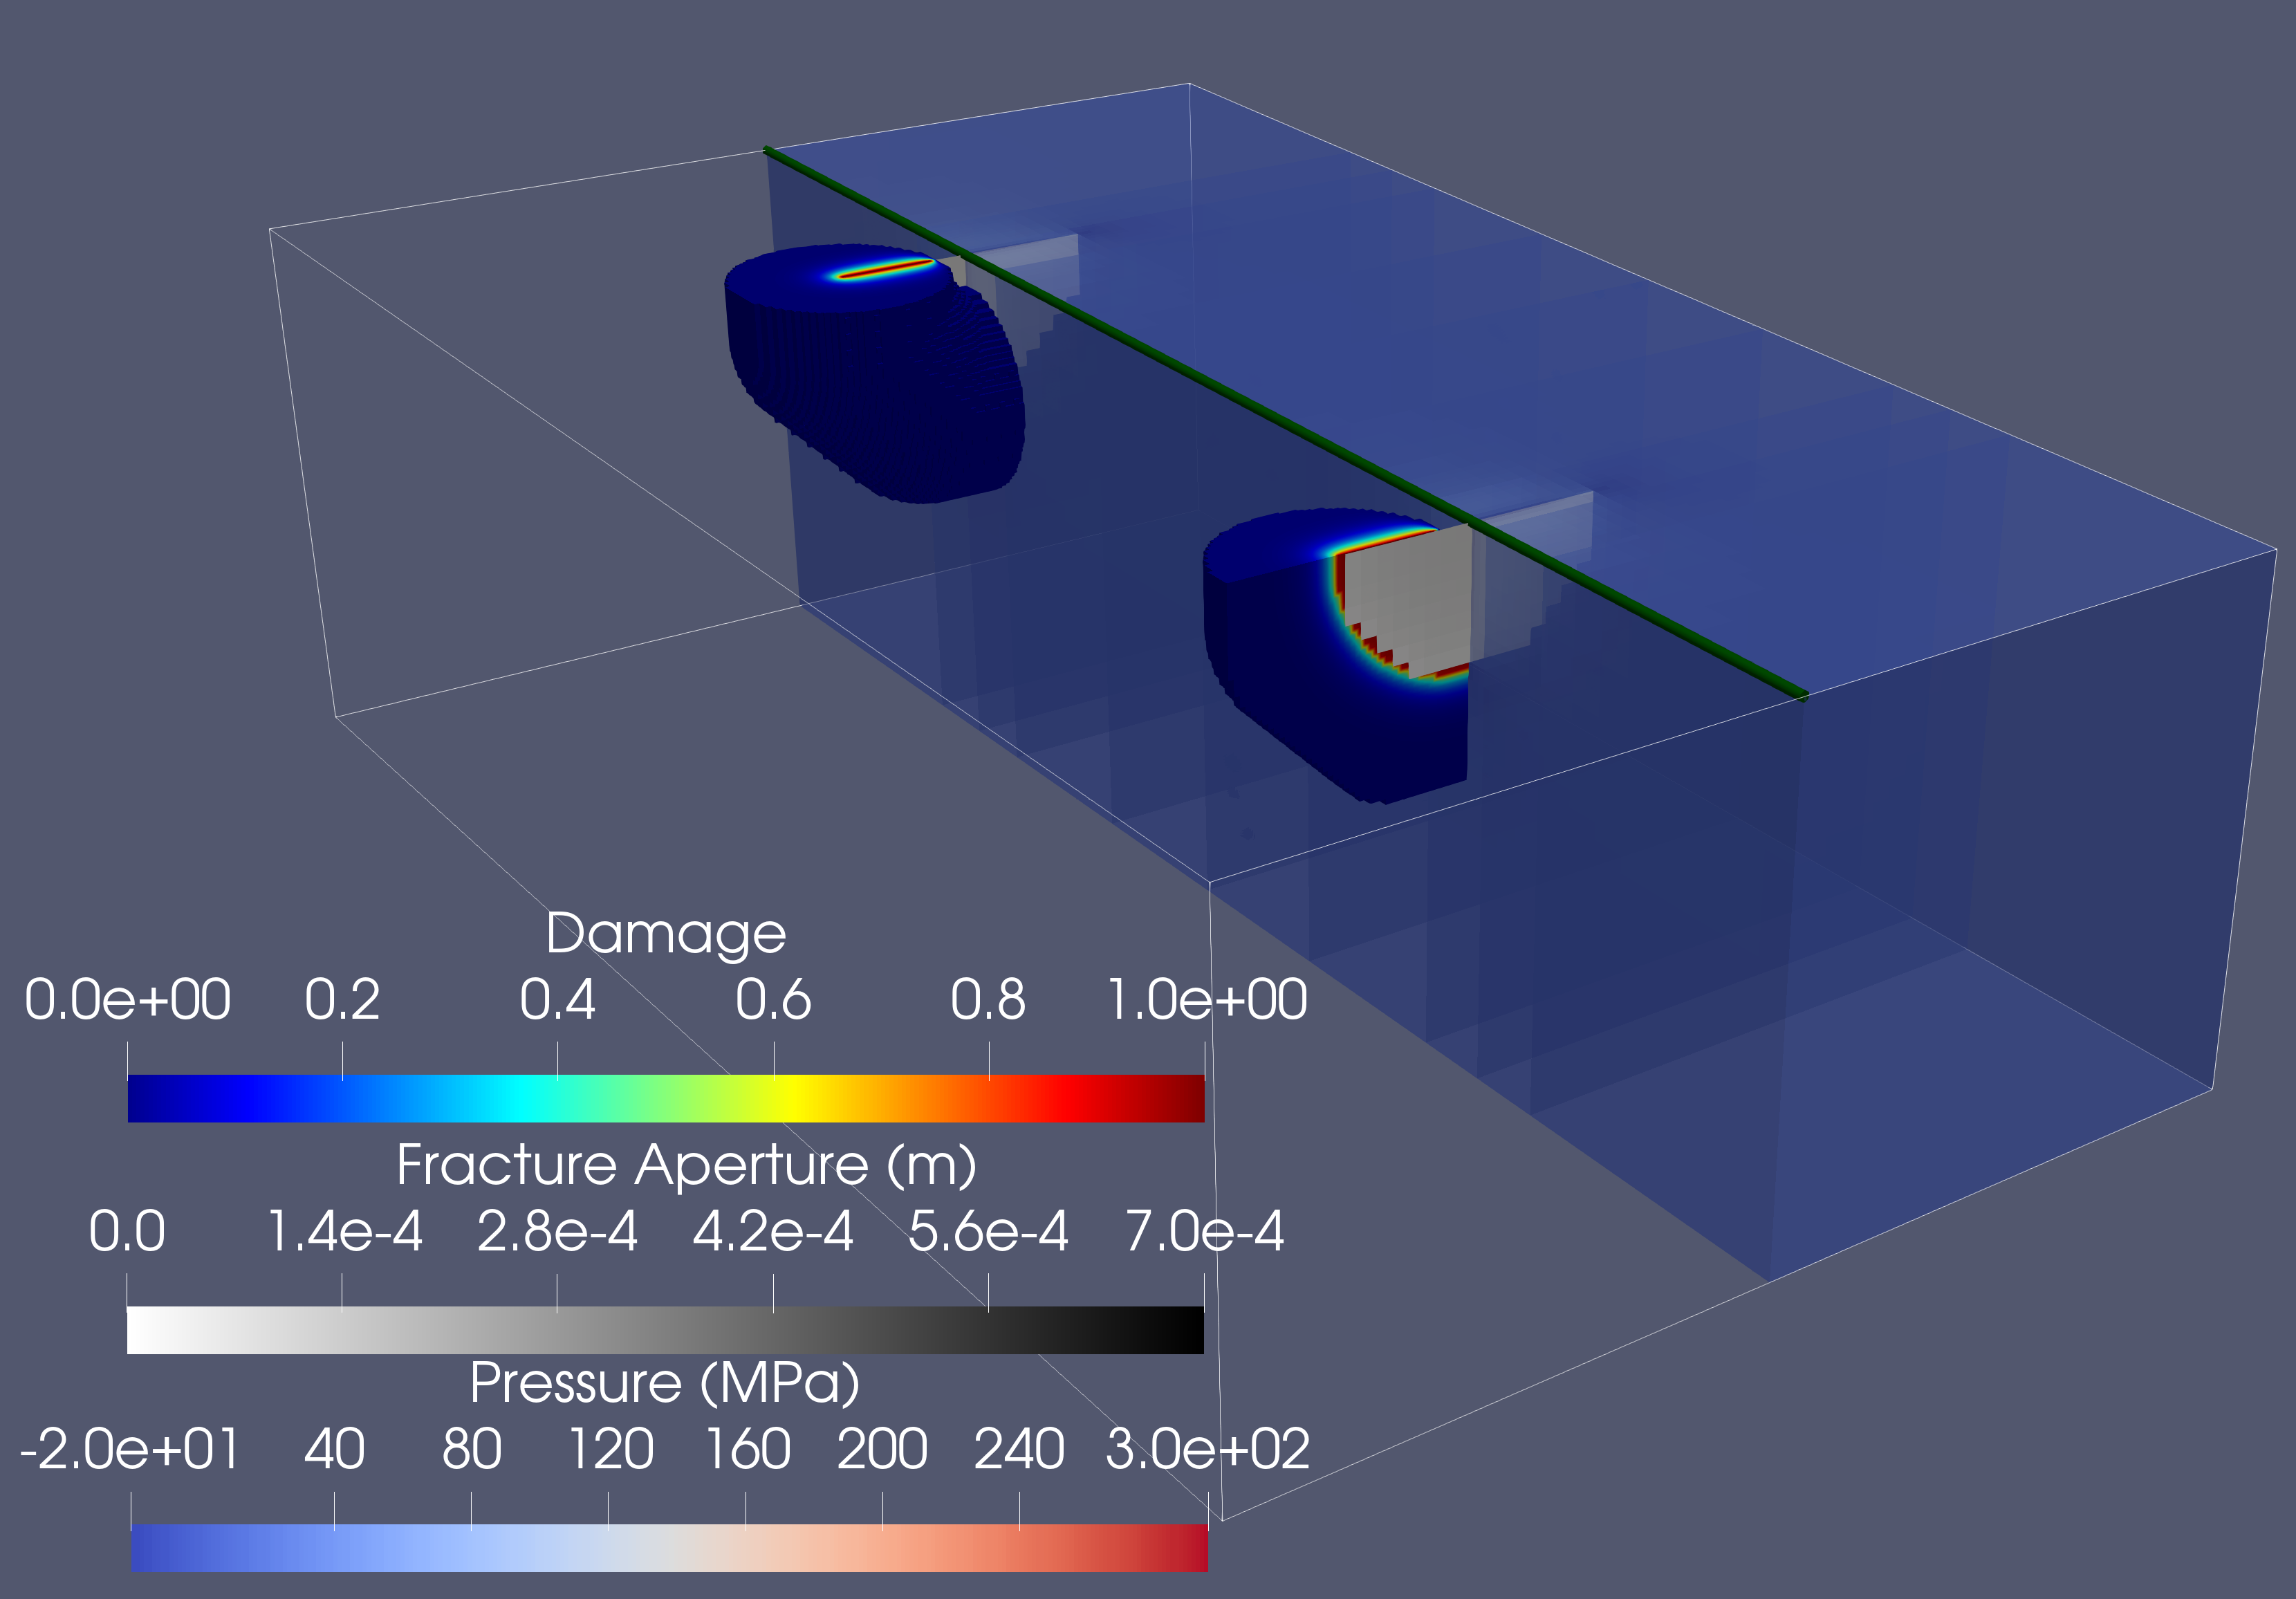
\includegraphics[width=\linewidth]{Chapter4/figures/3D/t_0.png}
  \caption{}
  \label{fig:parallel_t_0}
\end{subfigure}%
\hspace{1cm}
\begin{subfigure}{.45\textwidth}
  \centering
  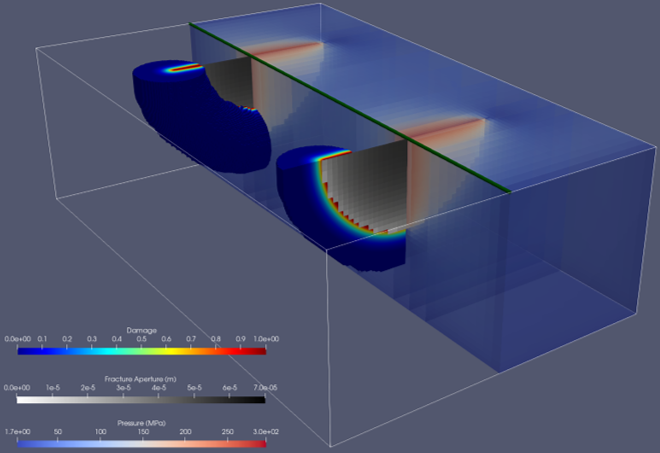
\includegraphics[width=\linewidth]{Chapter4/figures/3D/t_30.png}
  \caption{}
  \label{fig:parallel_t_1}
\end{subfigure}%

\bigskip
\begin{subfigure}{.45\textwidth}
  \centering
  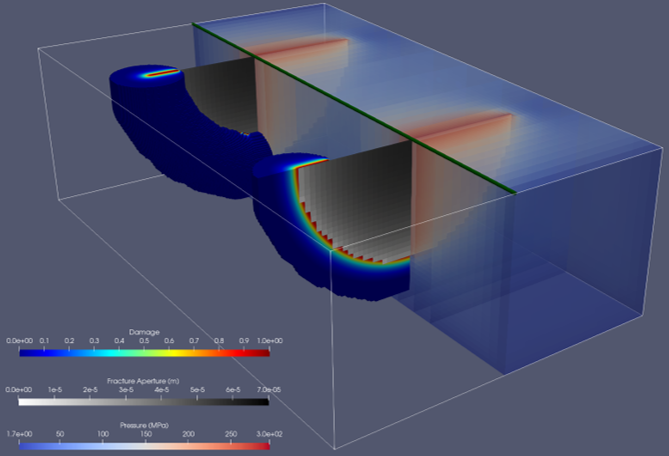
\includegraphics[width=\linewidth]{Chapter4/figures/3D/t_60.png}
  \caption{}
  \label{fig:parallel_t_2}
\end{subfigure}
\hspace{0.85cm}
\begin{subfigure}{.45\textwidth}
  \centering
  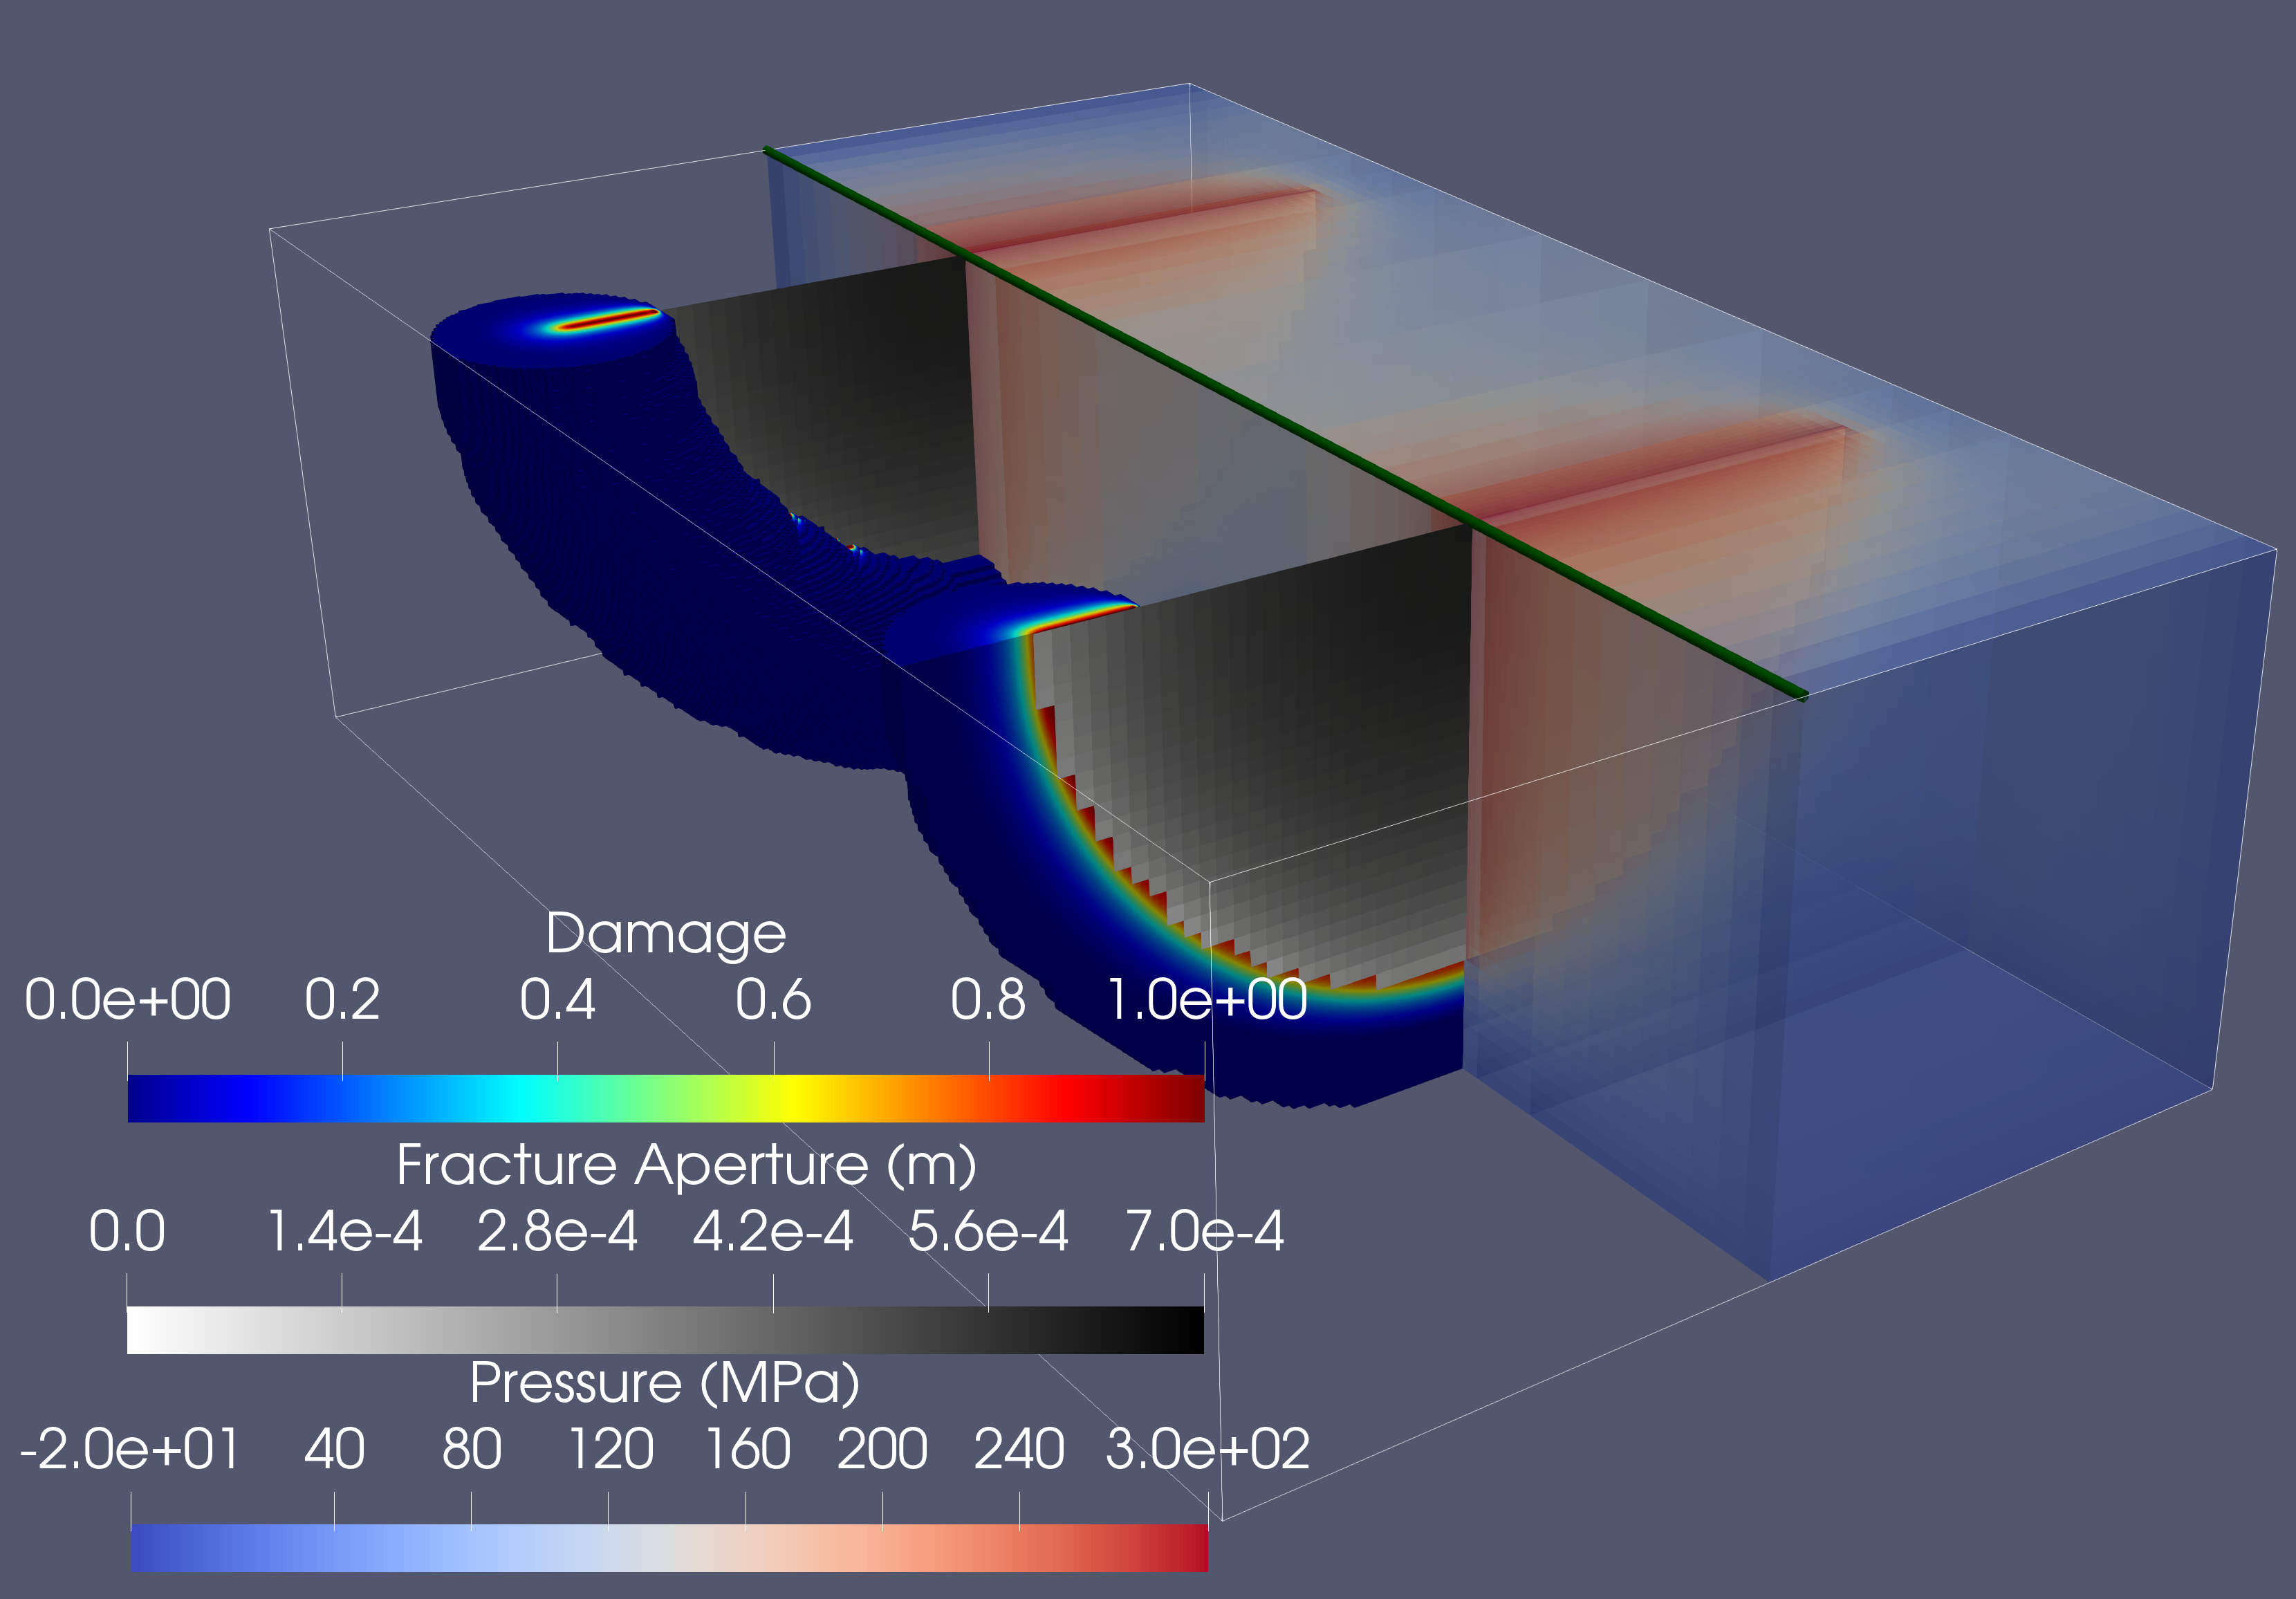
\includegraphics[width=\linewidth]{Chapter4/figures/3D/t_90.png}
  \caption{}
  \label{fig:parallel_t_3}
\end{subfigure}
  \caption{(a) time 1; (b) time 2; (c) time 3; and (d) time 4. } 
  \label{fig:parallel_snapshots}
\end{figure}

\begin{figure}[h]
\begin{subfigure}{.45\textwidth}
  \centering
  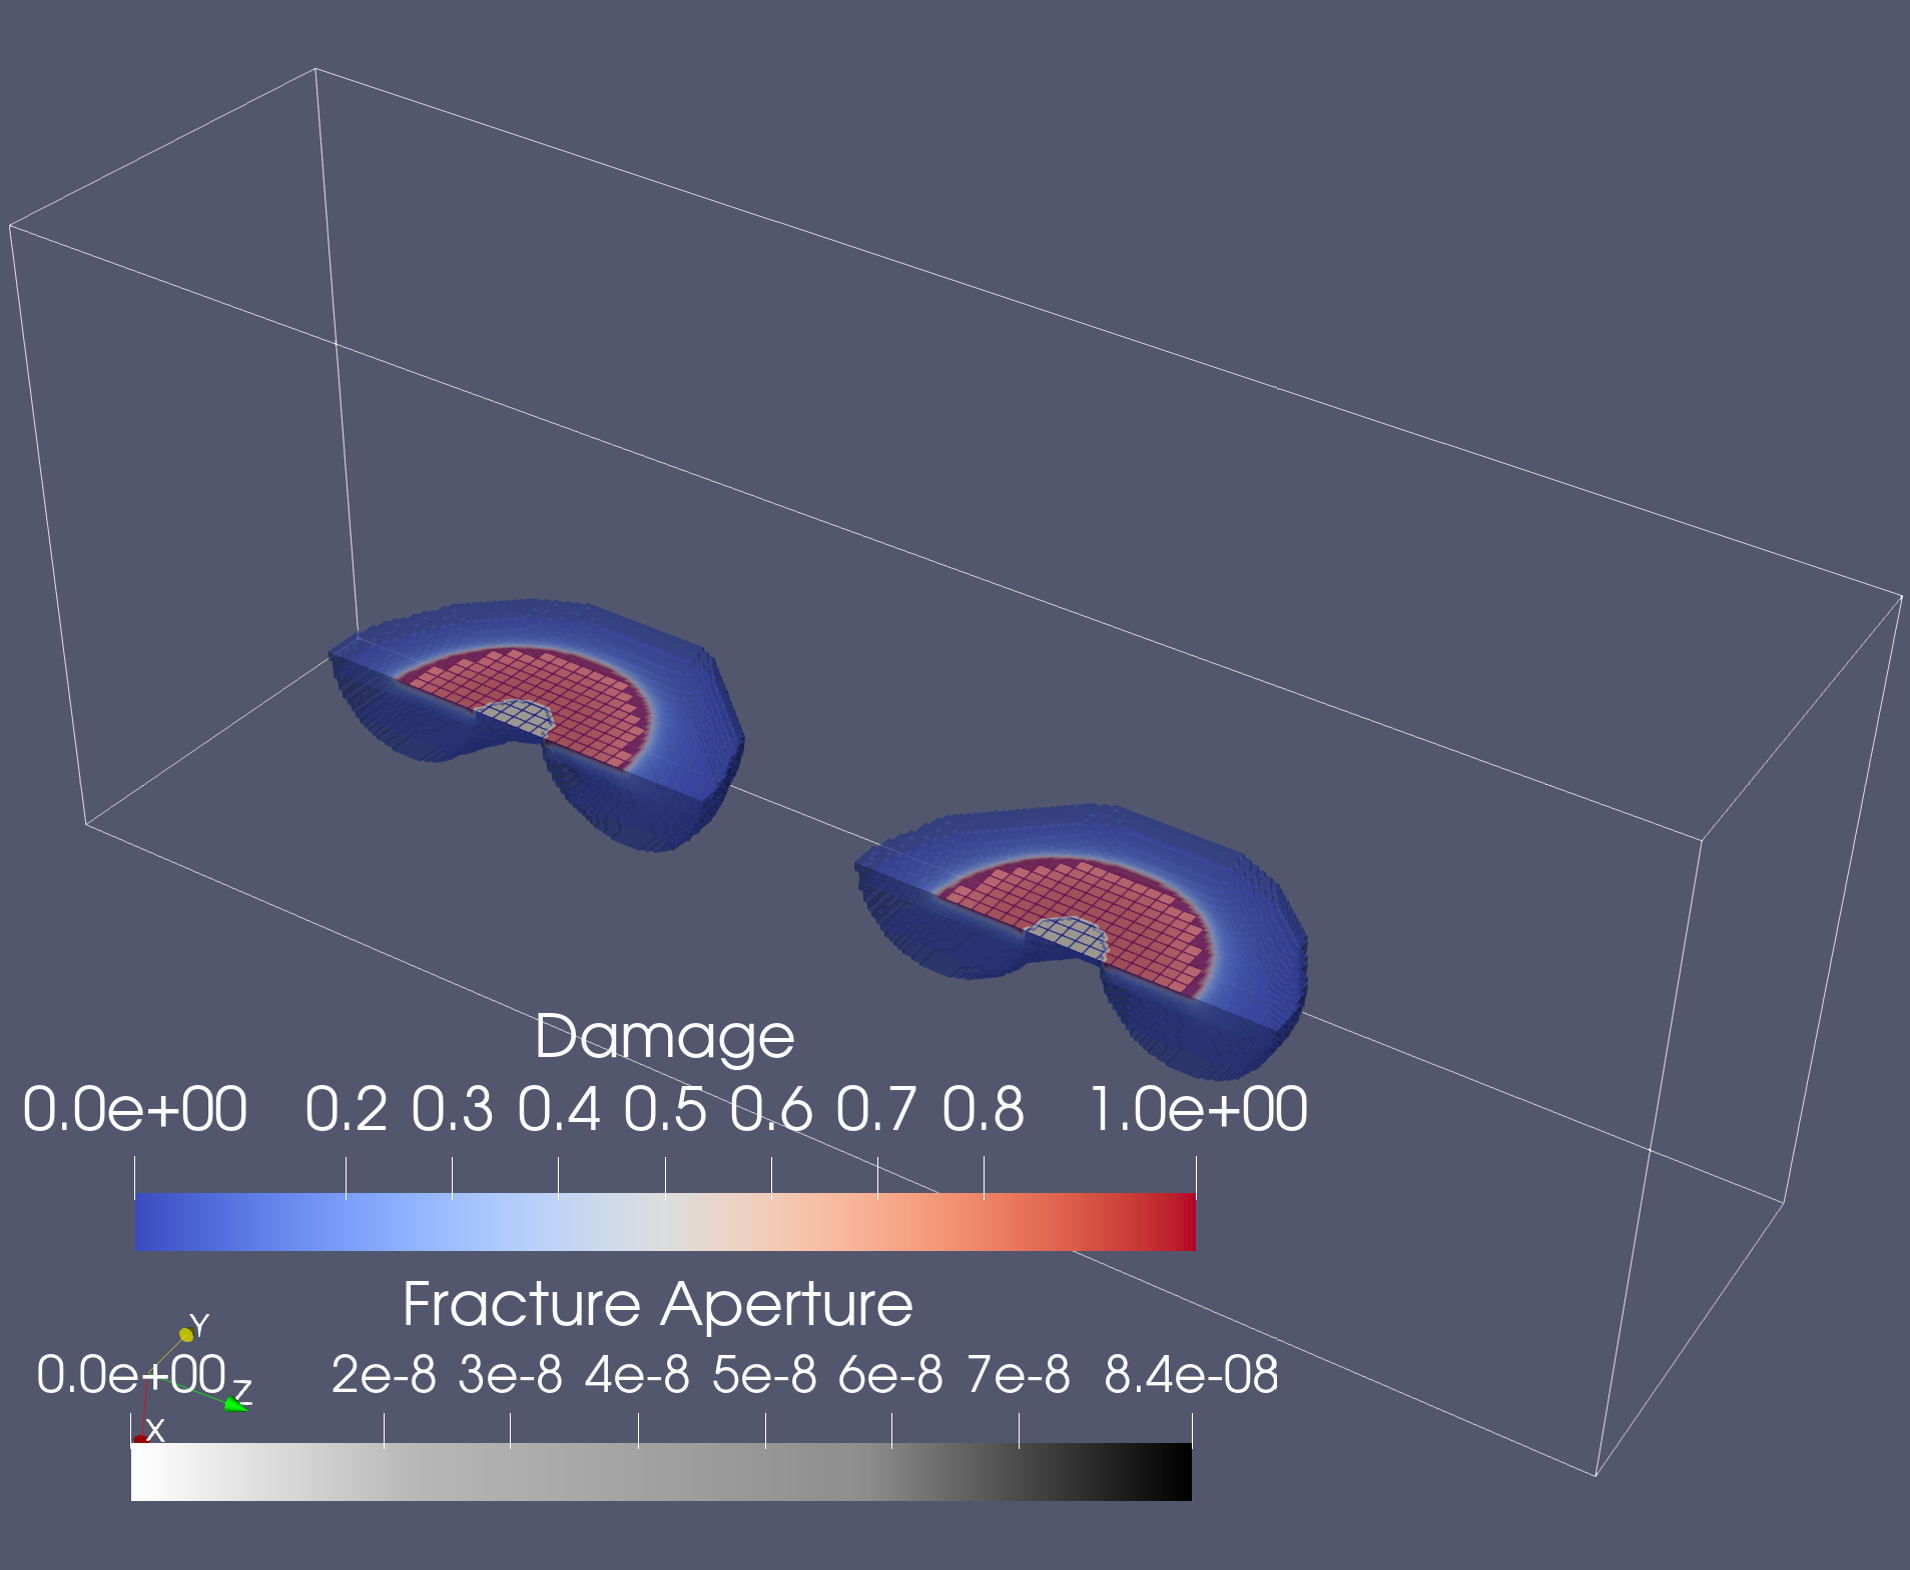
\includegraphics[width=\linewidth]{Chapter4/figures/merging/merge_t_1(1).png}
  \caption{}
  \label{fig:merge_t_0}
\end{subfigure}%
\hspace{1cm}
\begin{subfigure}{.45\textwidth}
  \centering
  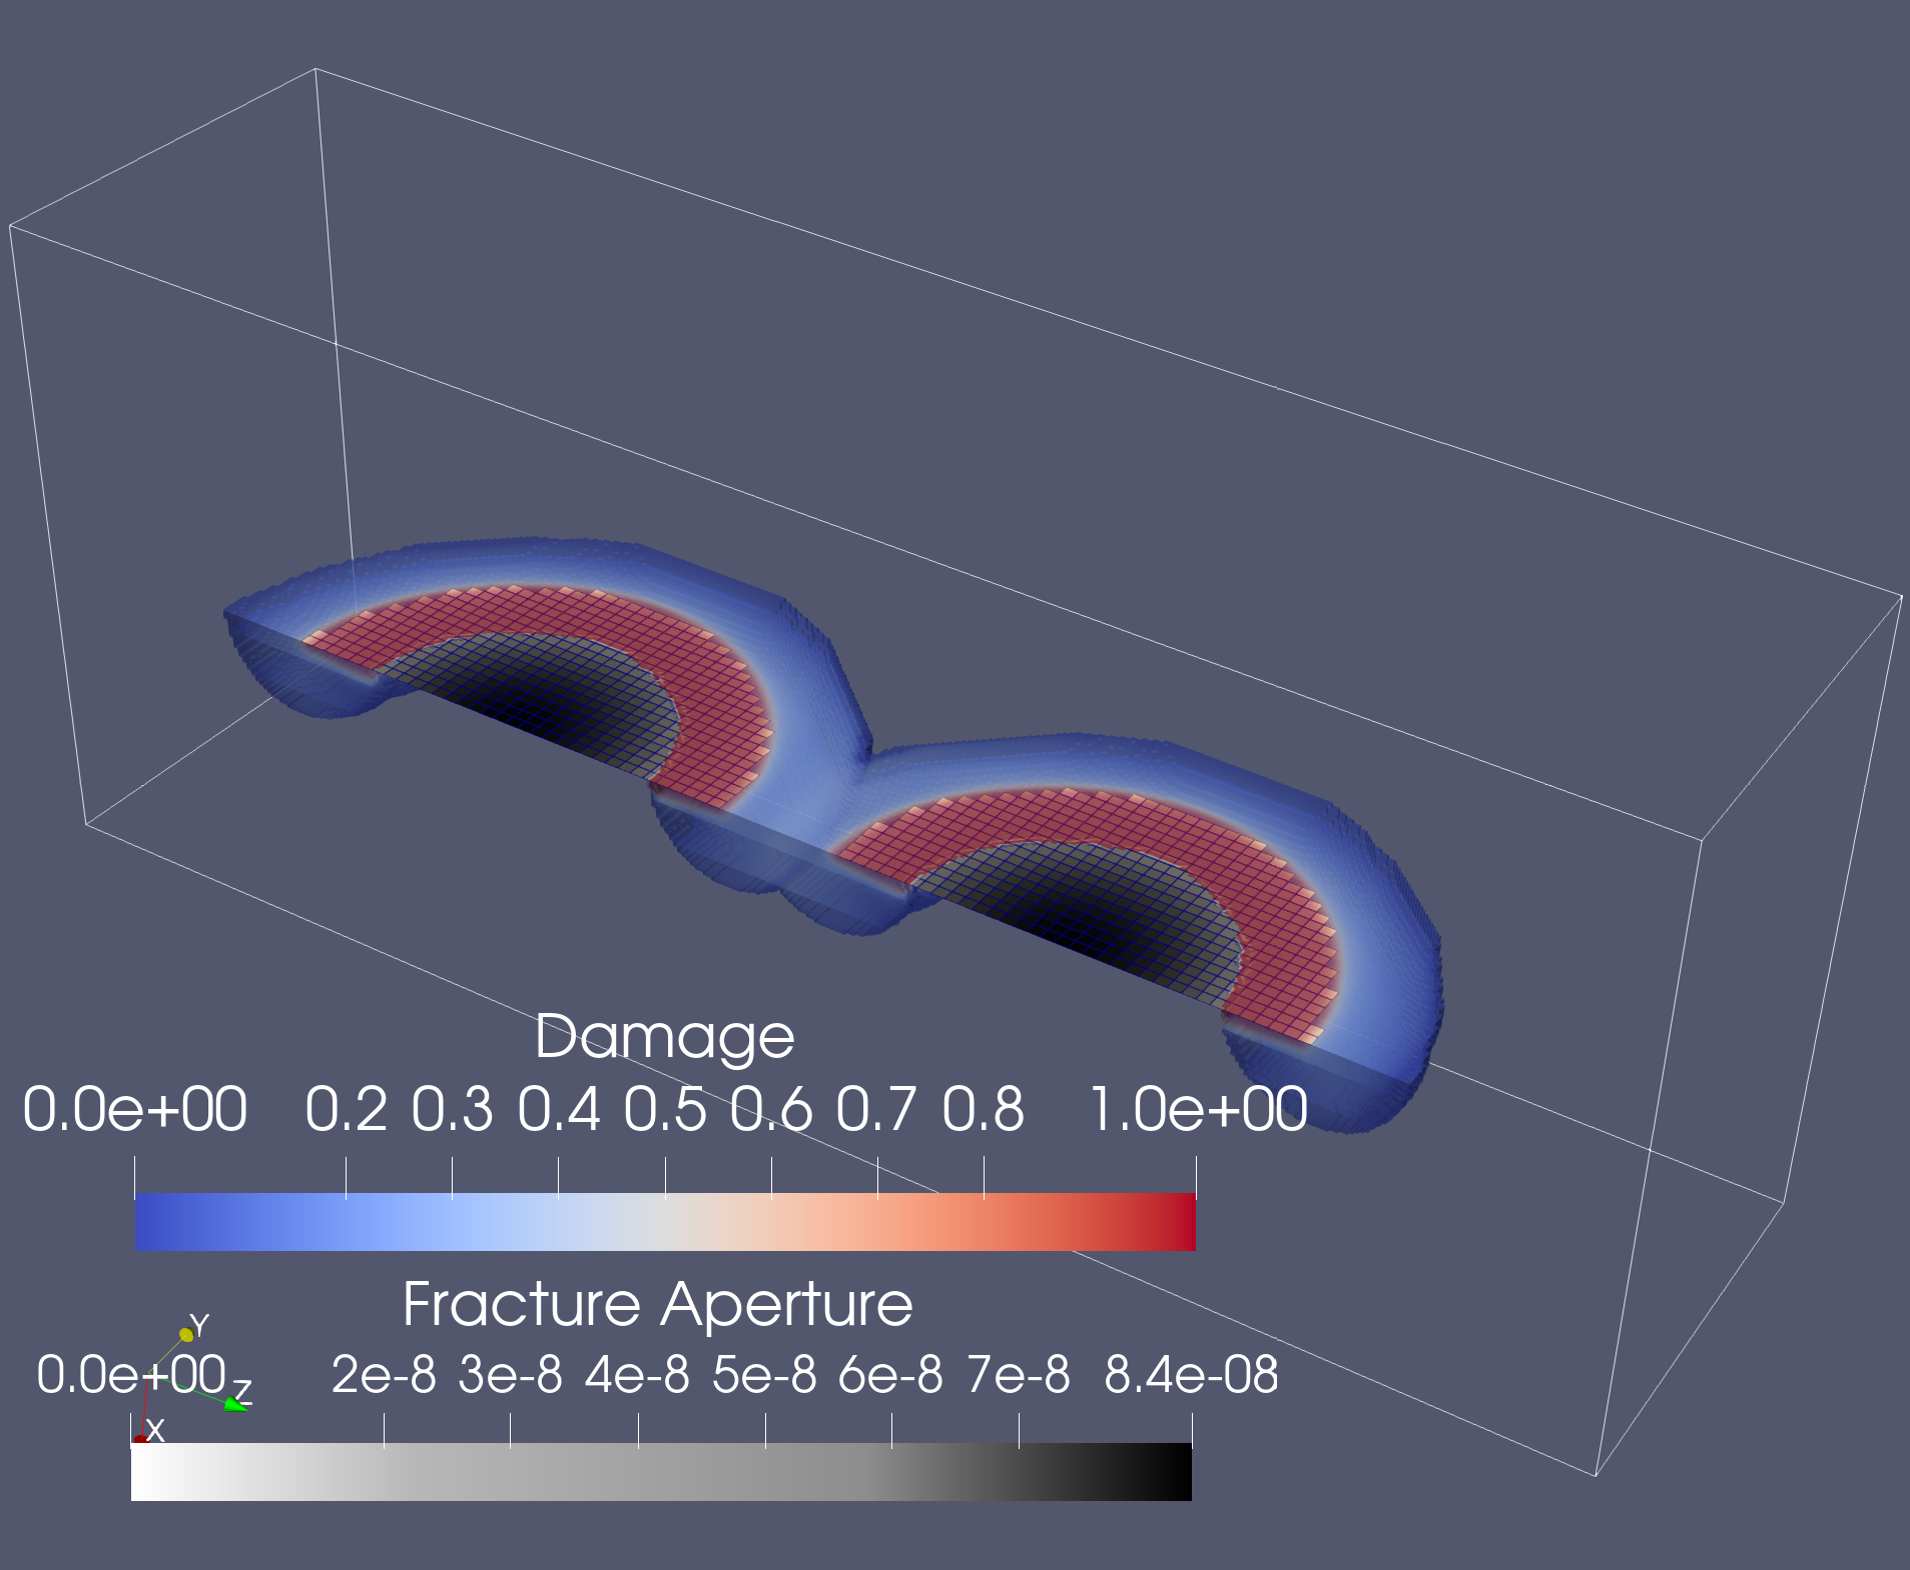
\includegraphics[width=\linewidth]{Chapter4/figures/merging/merge_t_17(1).png}
  \caption{}
  \label{fig:merge_t_1}
\end{subfigure}%

\bigskip
\begin{subfigure}{.45\textwidth}
  \centering
  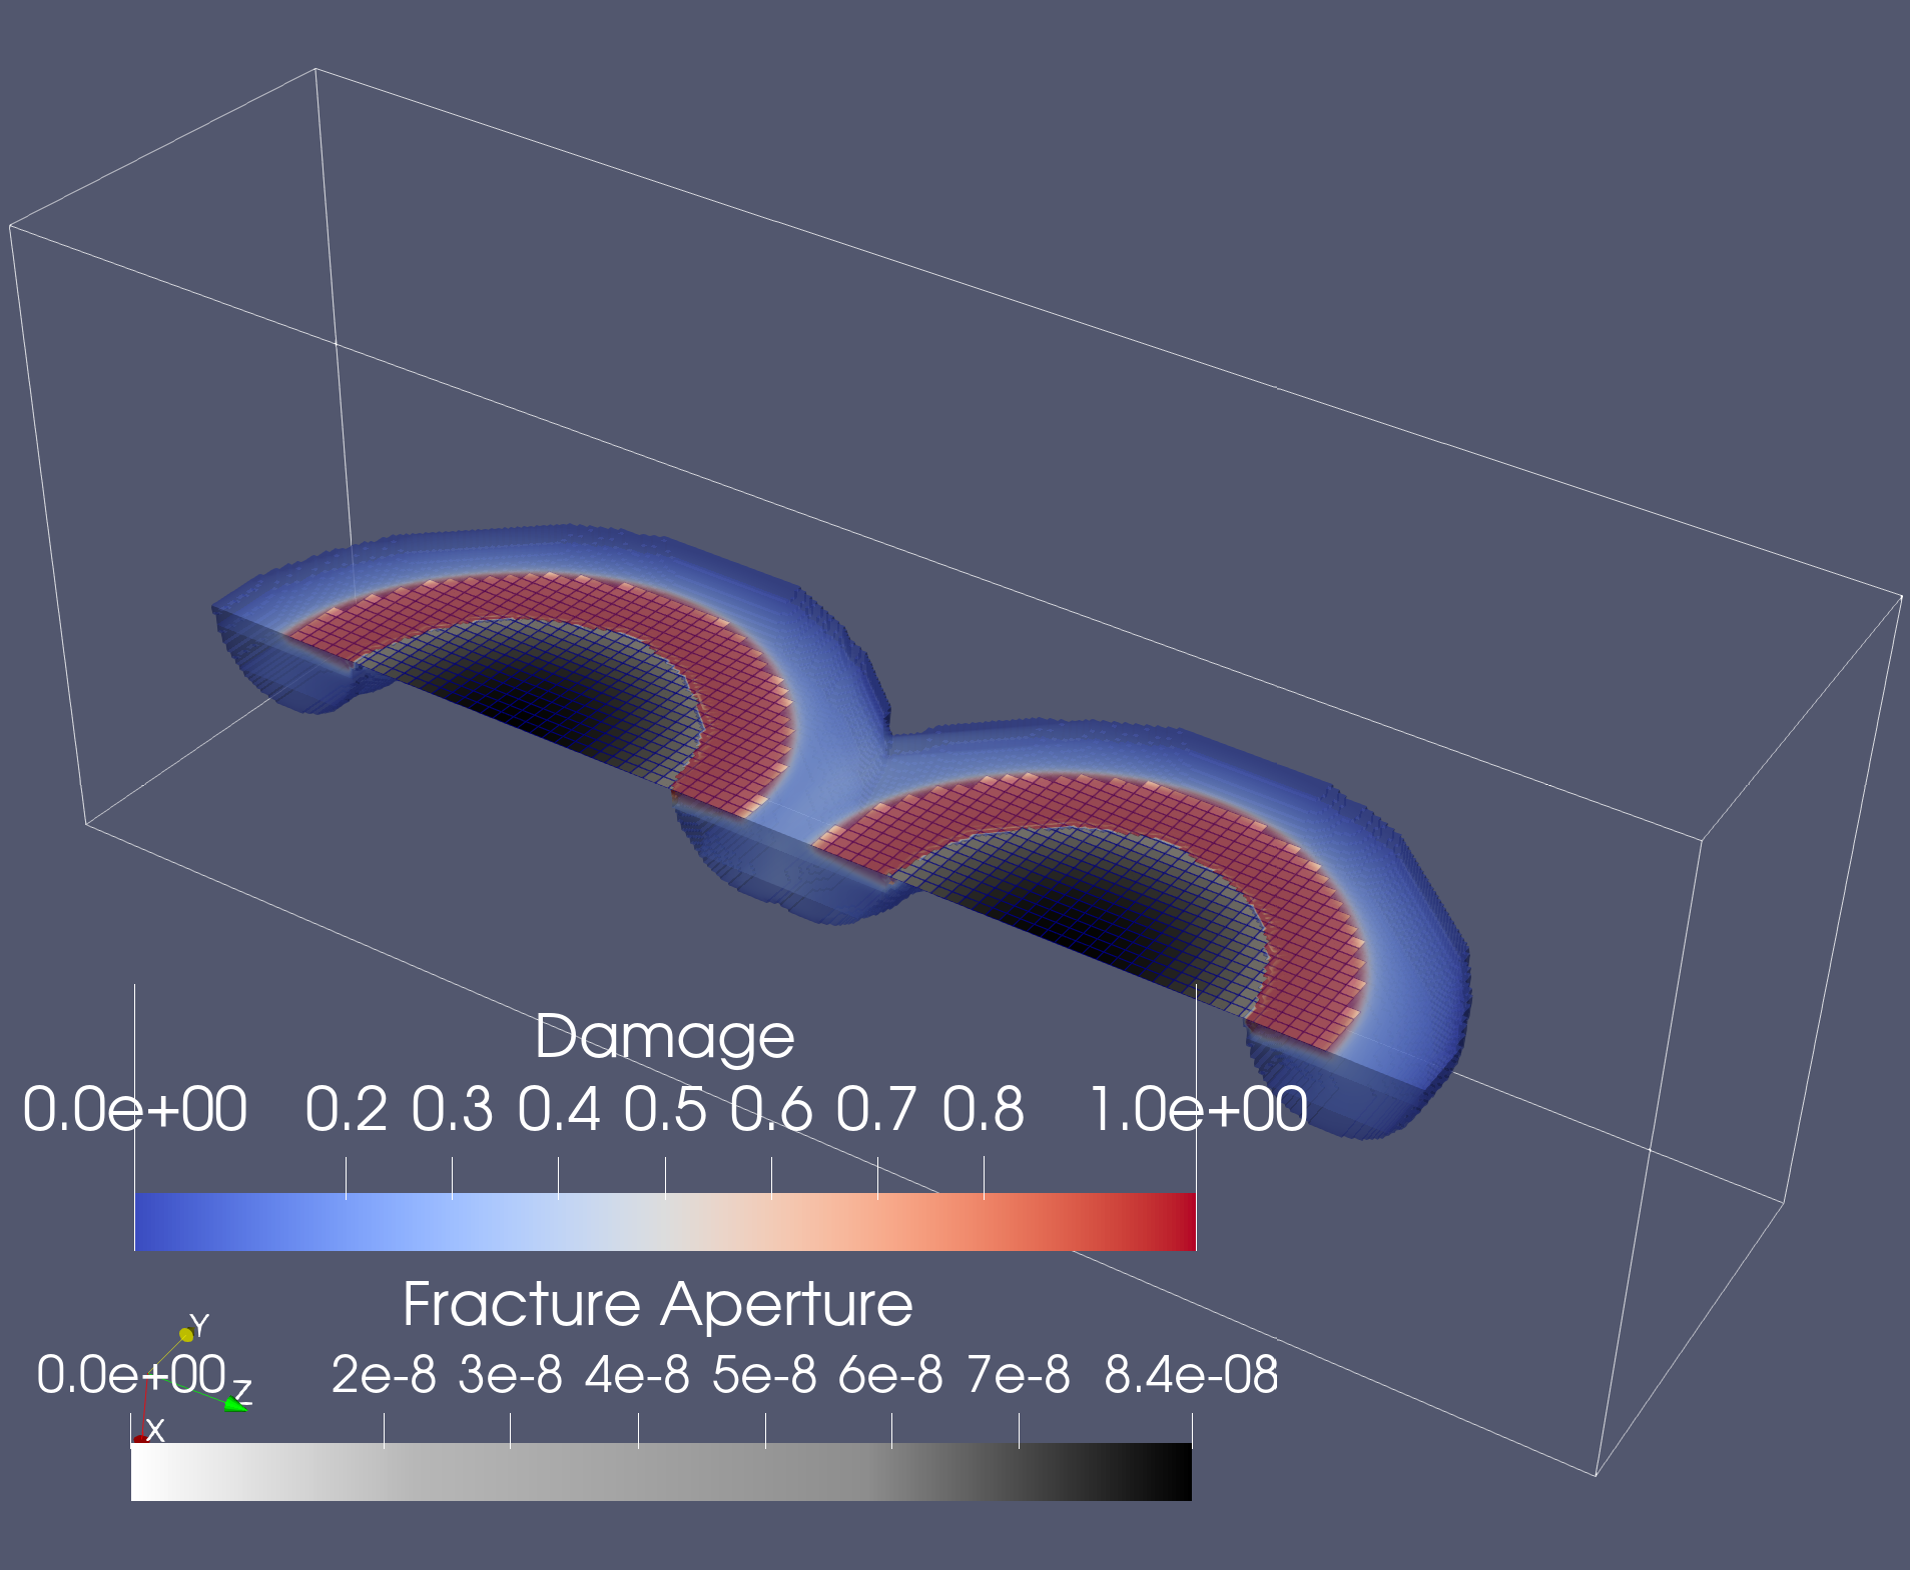
\includegraphics[width=\linewidth]{Chapter4/figures/merging/merge_t_23(1).png}
  \caption{}
  \label{fig:merge_t_2}
\end{subfigure}
\hspace{0.85cm}
\begin{subfigure}{.45\textwidth}
  \centering
  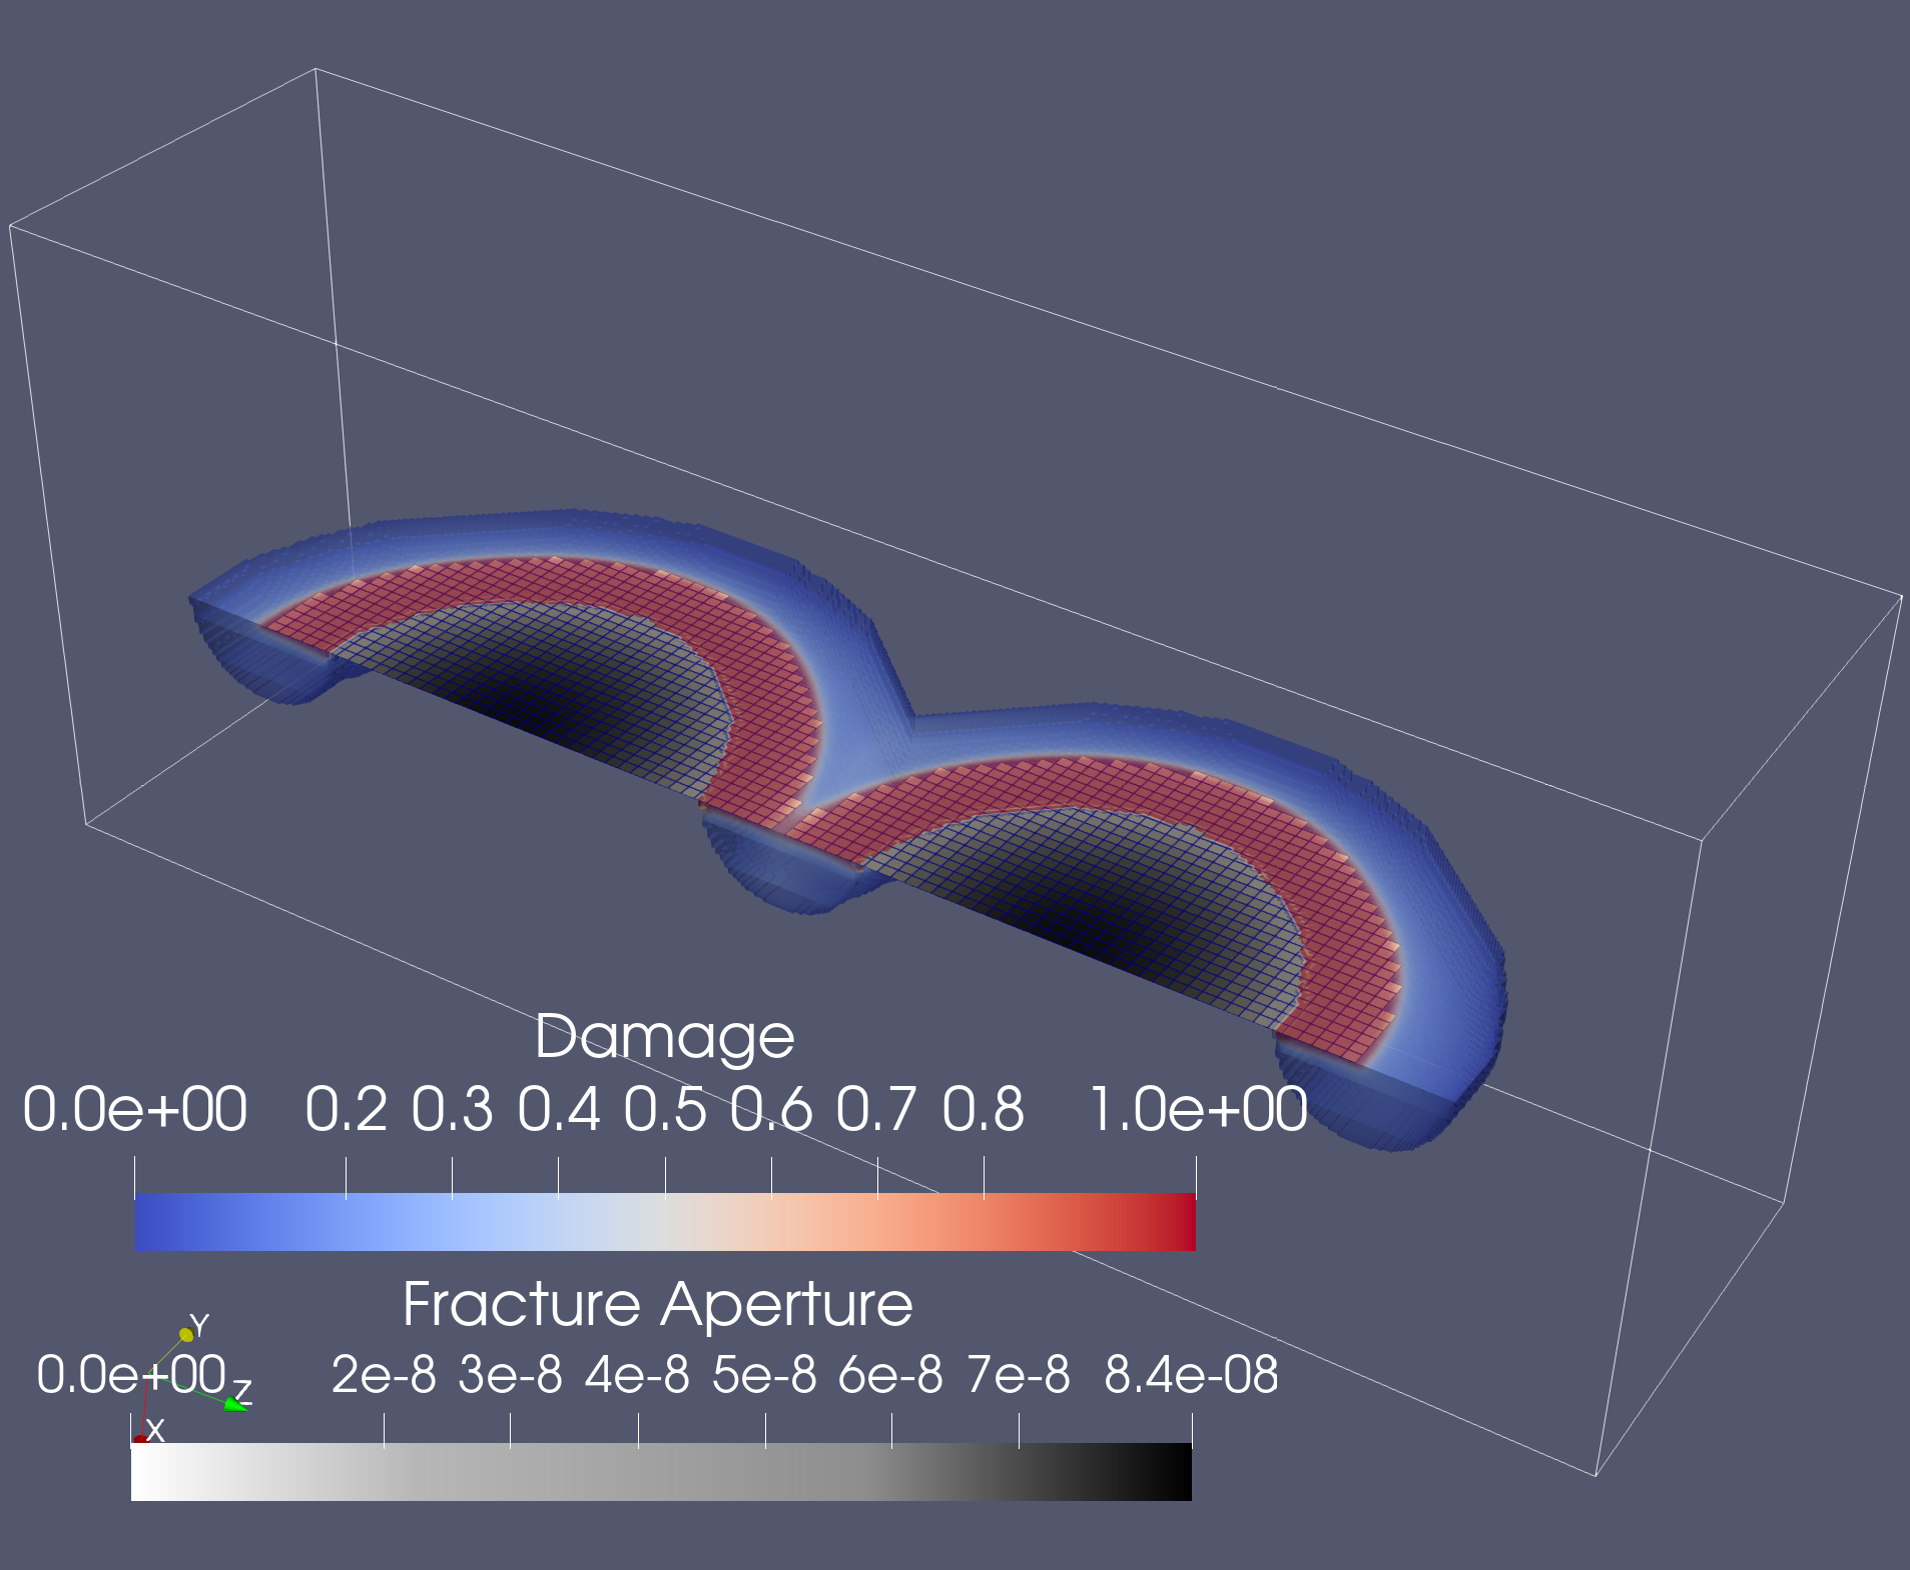
\includegraphics[width=\linewidth]{Chapter4/figures/merging/merge_t_34(1).png}
  \caption{}
  \label{fig:merge_t_3}
\end{subfigure}
  % \caption{(a) time 1; (b) time 2; (c) time 3; and (d) time 4. } 
  % \label{fig:parallel_snapshots}

\bigskip
\begin{subfigure}{.45\textwidth}
  \centering
  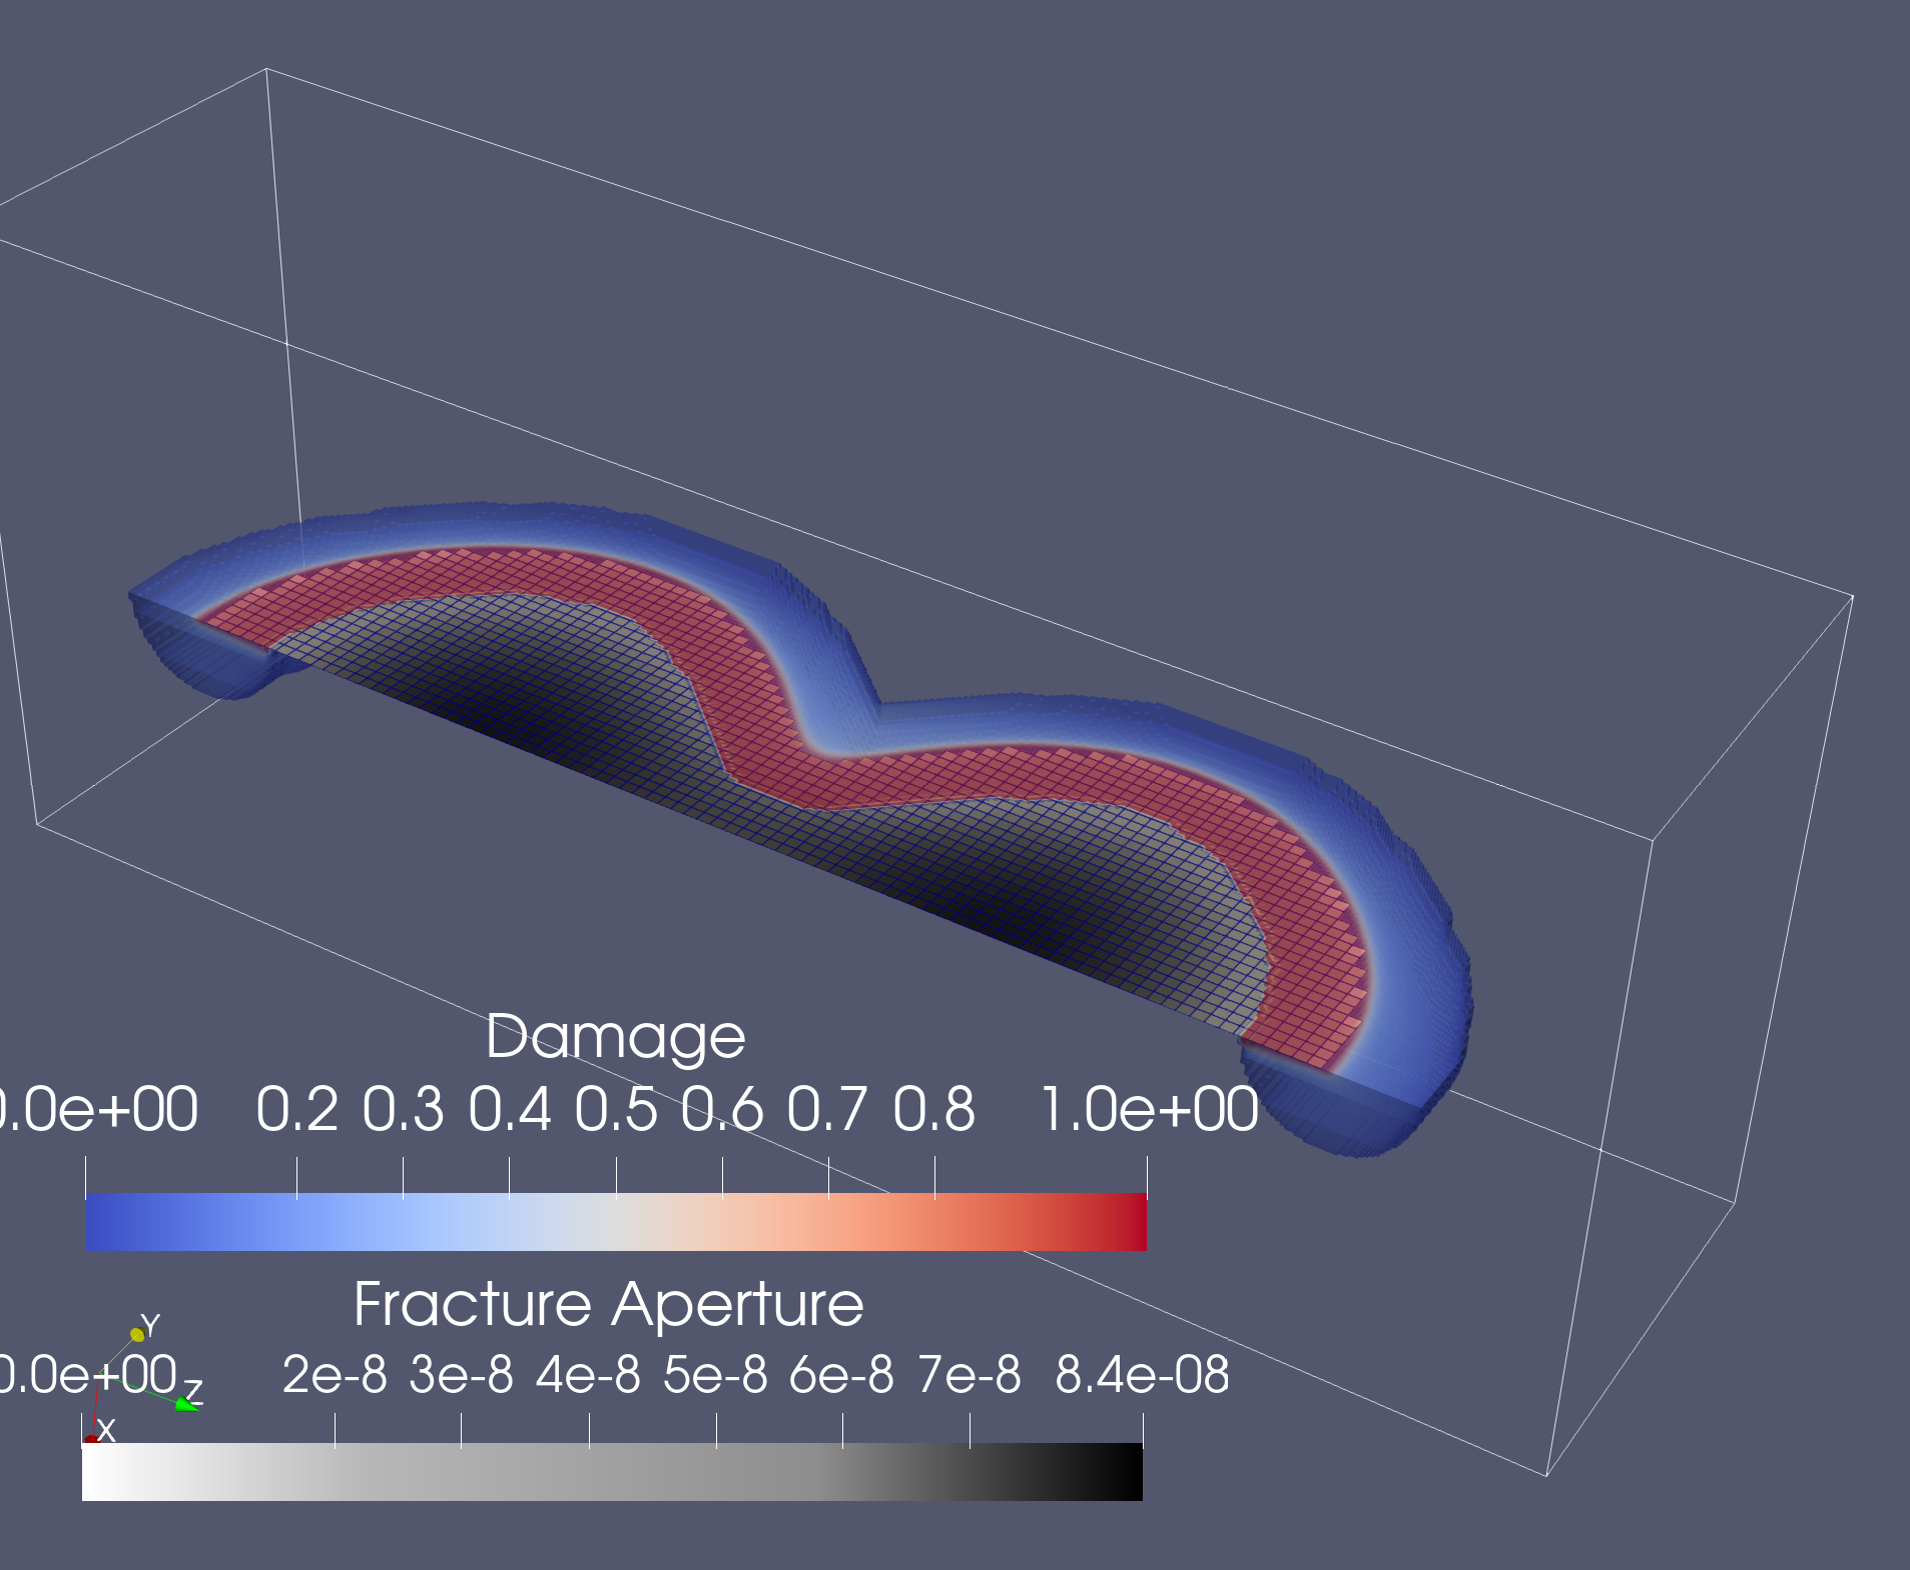
\includegraphics[width=\linewidth]{Chapter4/figures/merging/merge_t_45(1).png}
  \caption{}
  \label{fig:merge_t_4}
\end{subfigure}
\hspace{0.85cm}
\begin{subfigure}{.45\textwidth}
  \centering
  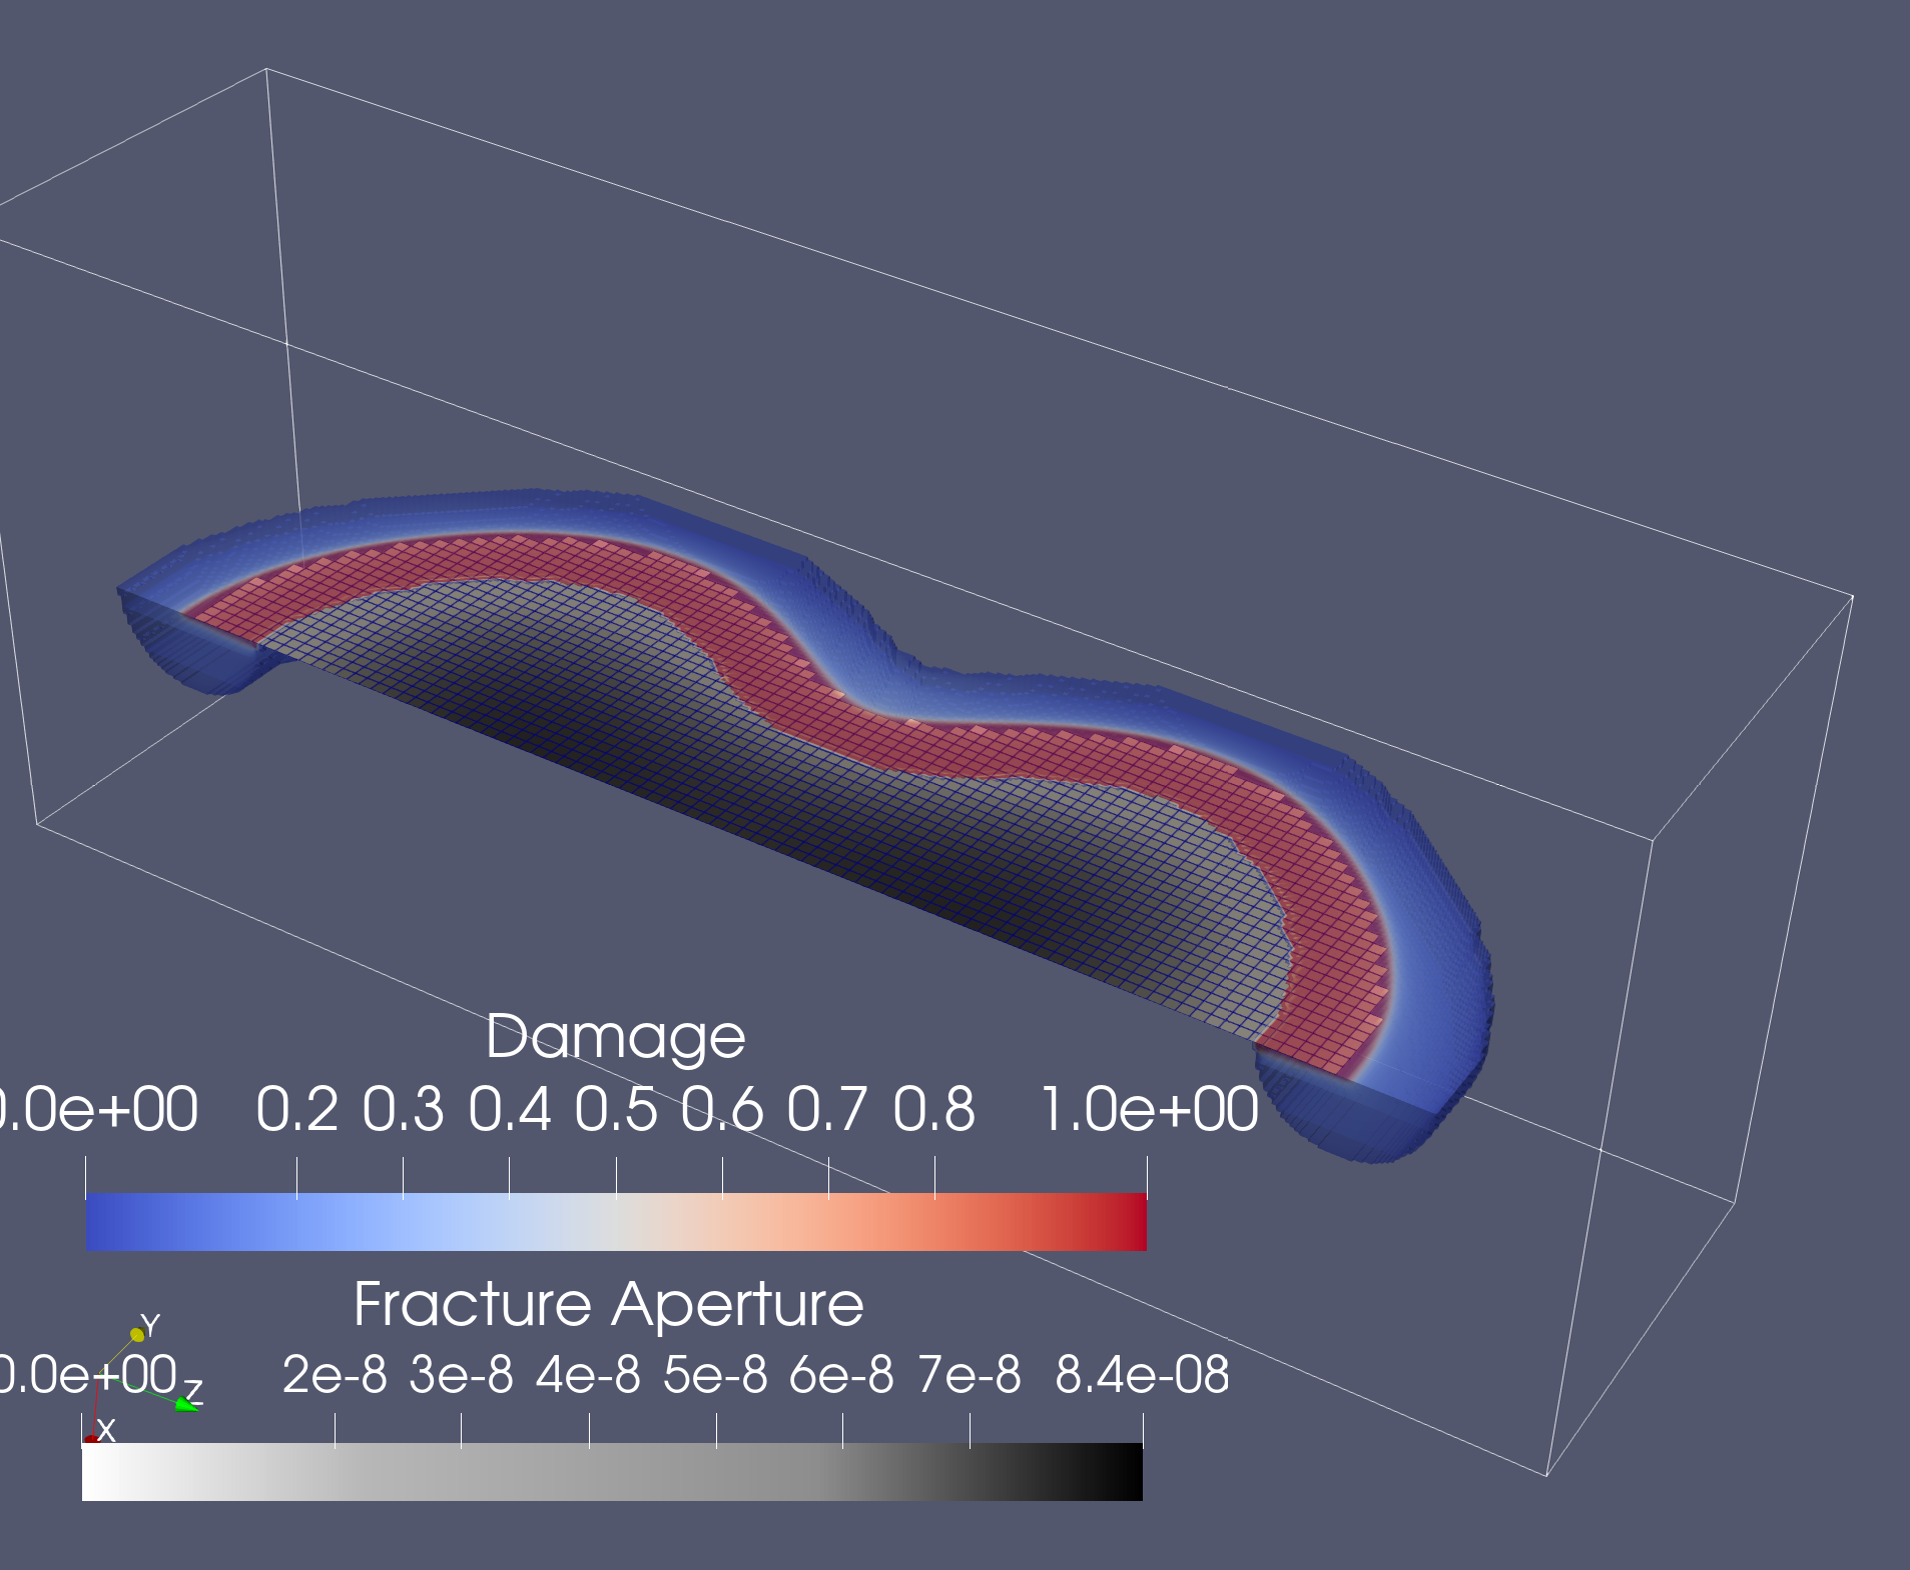
\includegraphics[width=\linewidth]{Chapter4/figures/merging/merge_t_67(1).png}
  \caption{}
  \label{fig:merge_t_5}
\end{subfigure}
  \caption{(a) time 1; (b) time 2; (c) time 3; and (d) time 4. } 
  \label{fig:merge_snapshots}  
\end{figure}

\begin{figure}[h]
% \centering
\begin{subfigure}{.45\textwidth}
  \centering
  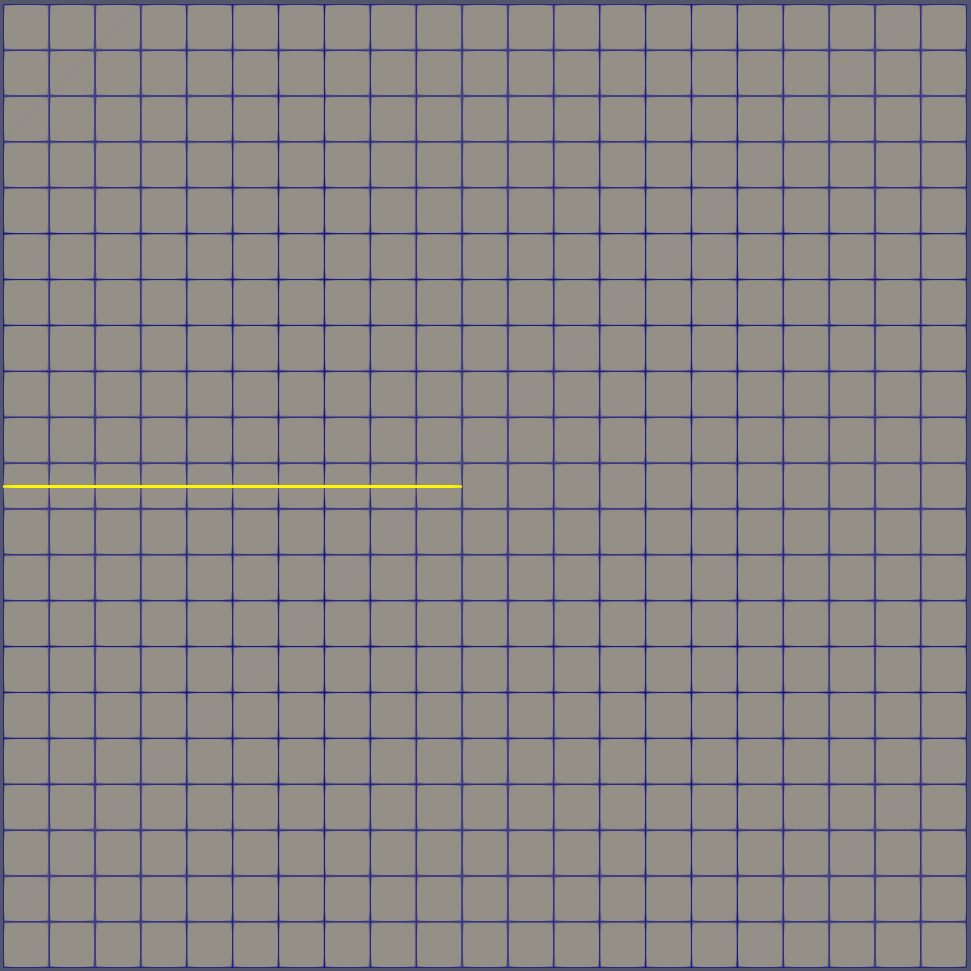
\includegraphics[width=0.765\linewidth]{Chapter4/figures/nonplanar/3D_example_init.png}
  \caption{}
  \label{fig:init_crack}
\end{subfigure}%
\begin{subfigure}{.54\textwidth}
  \centering
  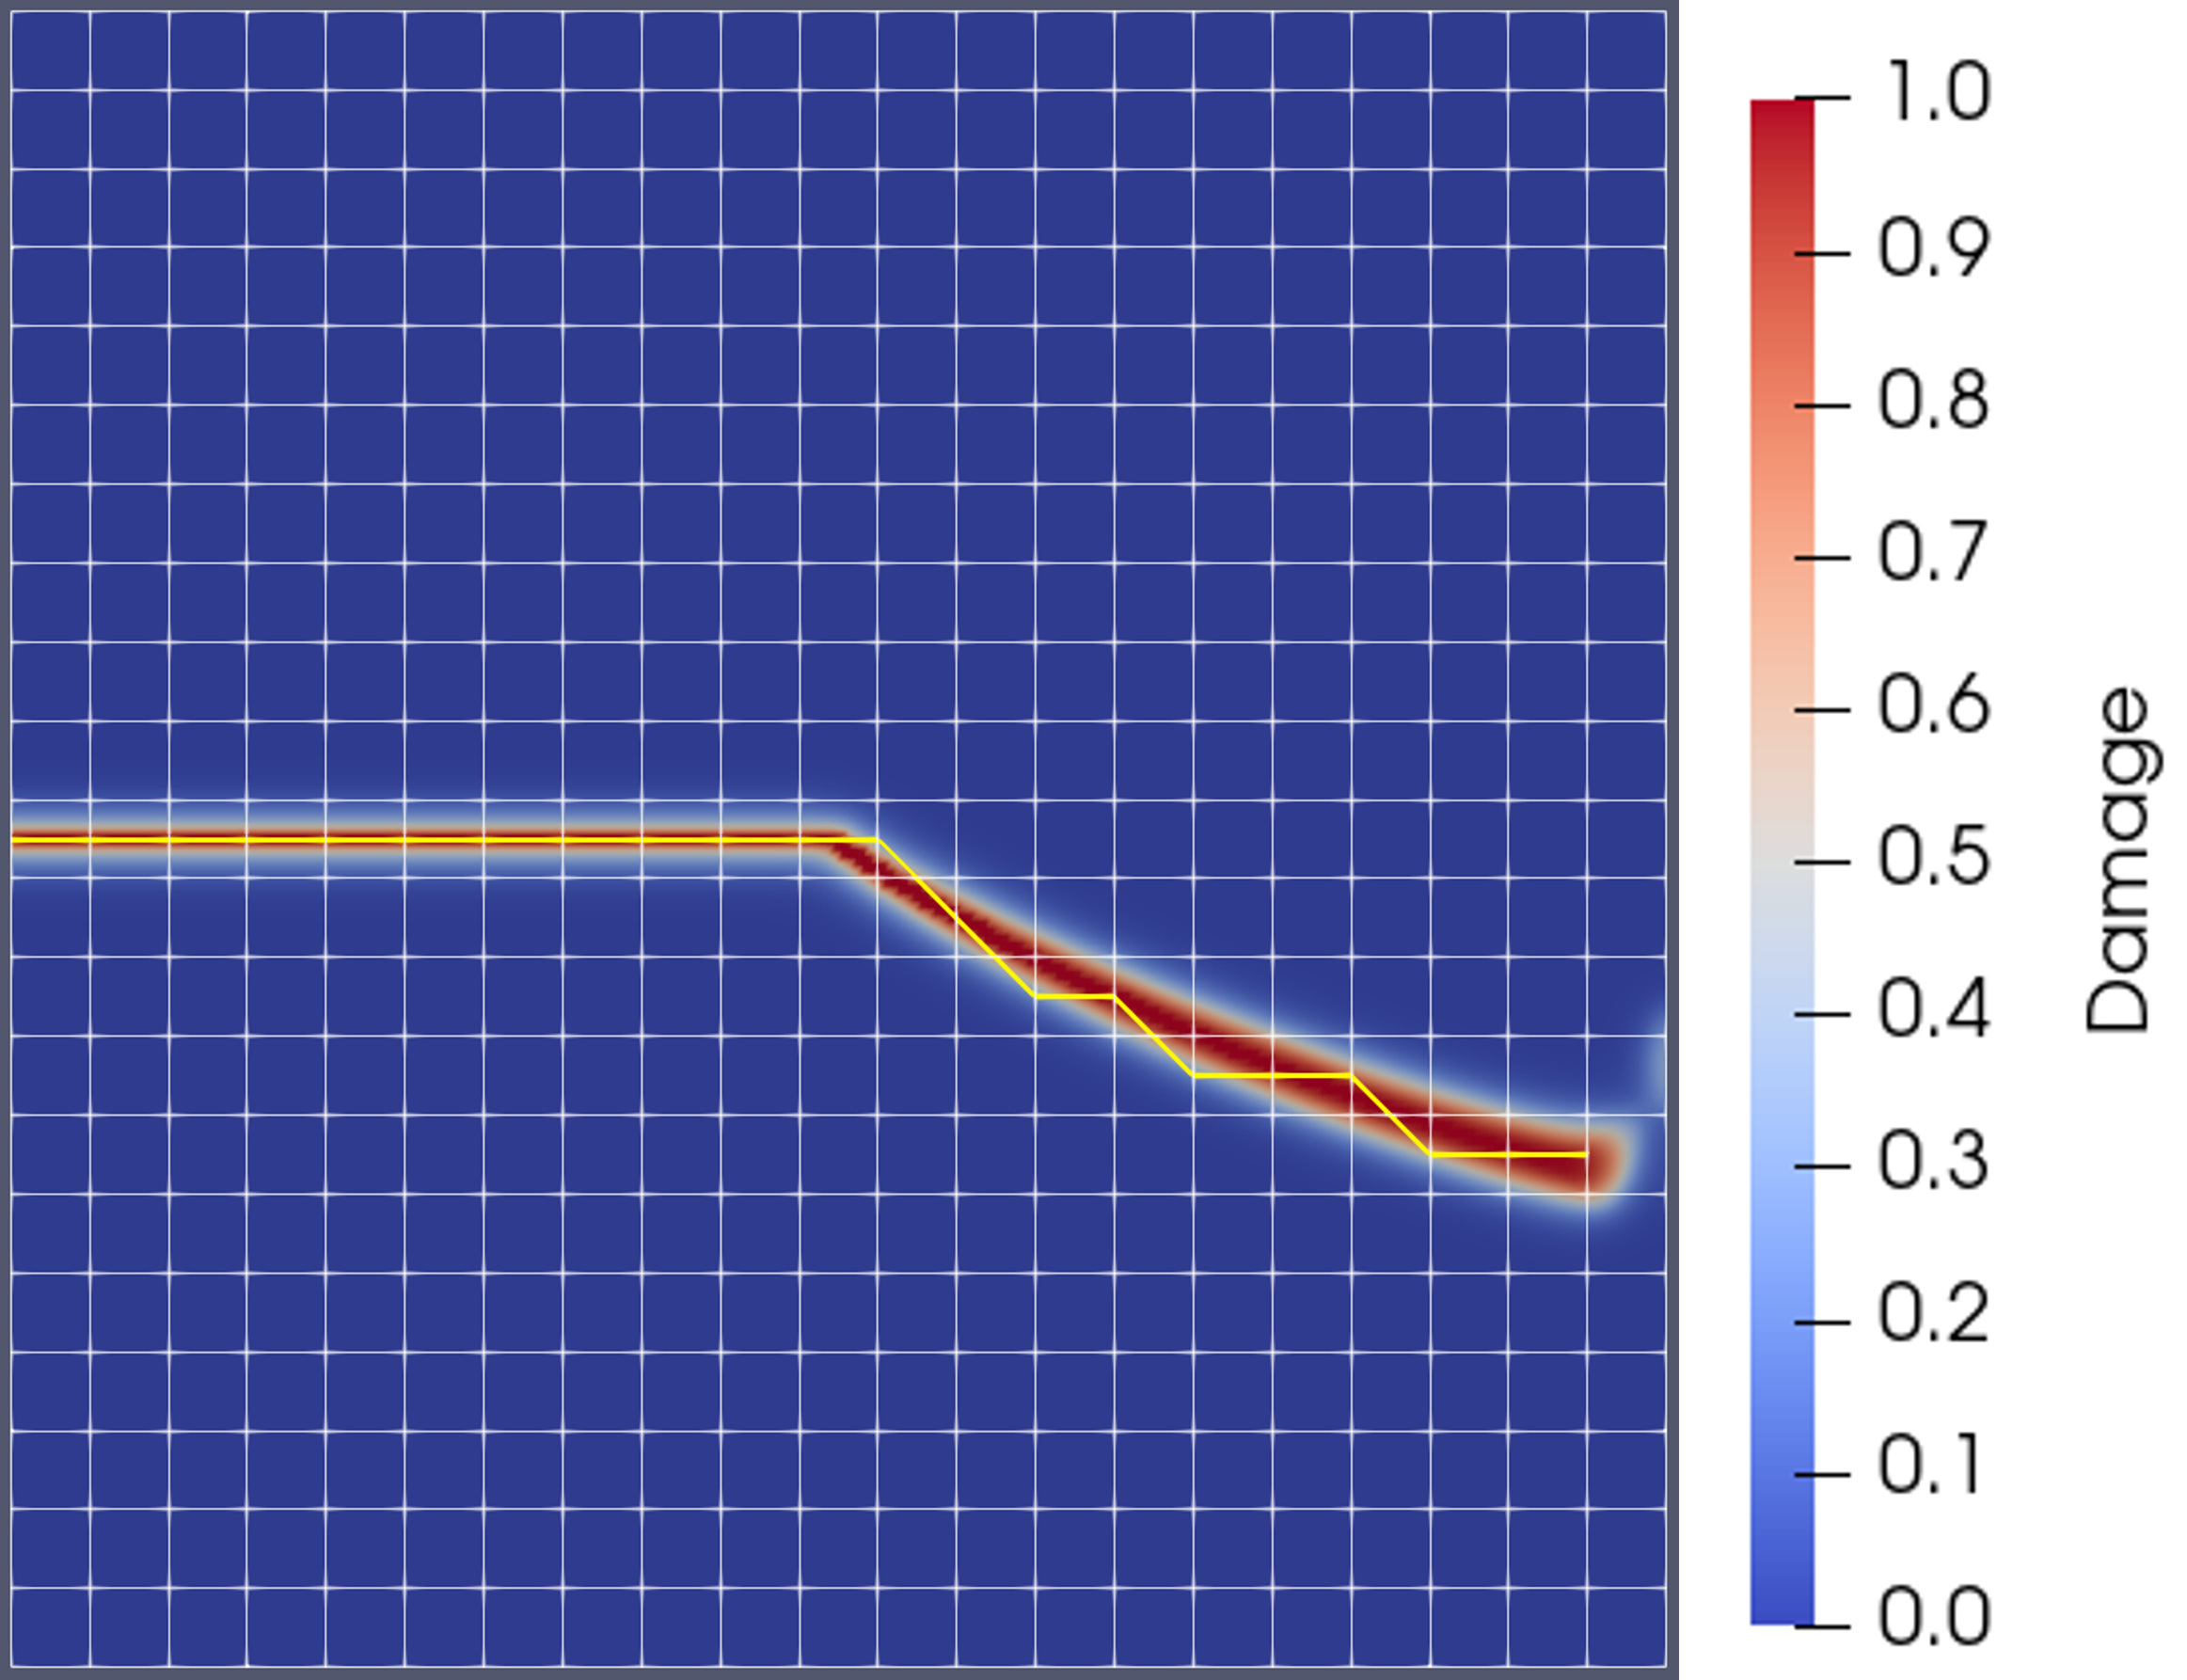
\includegraphics[width=0.83\linewidth]{Chapter4/figures/nonplanar/nonplanar_example.png}
  \caption{}
  \label{fig:crack_path}
\end{subfigure}%
  \caption{(a) Initial crack; (b) Final damage path.} 
  \label{fig:nonplanar_example}
\end{figure}